\documentclass[sigconf,nonacm]{acmart}
% Compile from this folder: pdflatex paper && pdflatex paper
% results_tables.tex is generated by `python paper/make_tables.py` (run from the repo root).
% Search for "TODO" before submitting: every red item still needs your input.
\usepackage{booktabs}
\usepackage{amsmath}
\usepackage{amssymb}
\newcommand{\todo}[1]{\textcolor{red}{\textbf{[TODO: #1]}}}
\settopmatter{printacmref=false}
\renewcommand\footnotetextcopyrightpermission[1]{}
\pagestyle{plain}

\begin{document}

\title{Traditional Retrieval Baselines for Scientific Search: TF-IDF and BM25 over arXiv Papers and Paragraphs}

\subtitle{Team NJMB \textbullet\ COS 487 Introduction to Information Retrieval, Course Project Part 1}

\author{Nicolas Borelli}
\affiliation{\institution{University of Southern Maine}\country{USA}}
\author{Jobe Odulio}
\affiliation{\institution{University of Southern Maine}\country{USA}}
\author{Mathieu Poulin}
\affiliation{\institution{University of Southern Maine}\country{USA}}
\author{Brady Roy}
\affiliation{\institution{University of Southern Maine}\country{USA}}

\begin{abstract}
We build a from-scratch search system for a collection of 34{,}308 arXiv papers from August and September 2024 and compare two classical ranking functions, TF-IDF with cosine normalization and Okapi BM25, at two granularities: whole papers (title and abstract) and individual paragraphs (2.28 million). Both models share one tokenizer and one set of inverted indexes, and a Flask search interface with filters and search history exposes them to users. On the 250 Study queries we report nDCG, nDCG@5, MRR, Precision@5 and Precision@10 (with lenient and strict relevance variants), average search time, and paired significance tests. BM25 is significantly better than TF-IDF for paragraph retrieval on every metric (nDCG 0.415 vs.\ 0.295, MRR 0.428 vs.\ 0.280, $p<0.001$), whereas at the paper level the two models are statistically indistinguishable (nDCG 0.360 vs.\ 0.344, $p=0.13$). Both models nearly fail on hard queries, which paraphrase the vocabulary of the relevant documents.
\end{abstract}

\maketitle

\section{Introduction}
Scientific search asks a system to connect short natural-language queries to long, technical documents. This project (Part 1 of three) builds the traditional baseline: TF-IDF and BM25 implemented without \texttt{scikit-learn}, \texttt{rank-bm25} or PyTerrier, together with a search interface and an evaluation harness. Later phases replace these models with neural and LLM-based retrievers, so the goal here is a reliable, well-understood reference point.

\paragraph{Collection.} The collection contains arXiv papers from August and September 2024. Each paper is provided as raw HTML (from ar5iv) and as a processed JSON record with \texttt{paper\_id}, \texttt{title}, \texttt{abstract} and \texttt{paragraphs}. We use the JSON records: 34{,}308 papers containing 2{,}275{,}574 paragraphs. All 34{,}308 files parse, so no record is skipped at load time.

\paragraph{Tasks.} \emph{Paper retrieval} returns paper IDs (format YYMM.NNNNN); \emph{paragraph retrieval} returns paragraph IDs from the JSON files. For each query the system returns the top 100 results in 6-column TREC format. Three query files are provided: \texttt{Train.json} (2{,}000 queries), \texttt{Study.json} (250 queries, qrels provided) and \texttt{Test.json} (250 queries, qrels withheld). Each file is 30\% easy, 50\% medium and 20\% hard. All analysis in this paper uses the Study queries; they were not used for tuning, and neither was \texttt{Train.json}, because both models run with default parameters. Relevance is 2 (fully relevant), 1 (partially relevant), and 0 for anything not in the qrels. The Study qrels are sparse: on average 1.56 judged papers per query (390 judgments) and 2.91 judged paragraphs per query (728 judgments).

\paragraph{Contributions.} (1) A shared tokenizer and index feeding both models; (2) TF-IDF and BM25 scorers written from the formulas; (3) a search interface with highlighting, filters, search history and an annotation page; (4) an evaluation script with paired significance tests; (5) an analysis of where each model succeeds and fails.

\section{Methodology}
\subsection{Pre-processing and indexing}
All text, for documents and queries alike, passes through one tokenizer. It strips any HTML markup with BeautifulSoup (\texttt{html.parser}), lowercases, extracts alphabetic tokens with the regular expression \verb|\b[a-z]+\b|, and removes NLTK's 198 English stop words. No stemming or lemmatization is applied. Because \verb|\b| treats digits, underscores and accented letters as word characters, any token that mixes letters with one of these is discarded entirely rather than trimmed: ``3D'', ``L2'', ``x\_1'' and ``Schr\"odinger'' produce no token at all, while hyphens do split (``GPT-4'' $\rightarrow$ \texttt{gpt}, ``state-of-the-art'' $\rightarrow$ \texttt{state}, \texttt{art}). As an efficiency measure, text containing neither \texttt{<} nor \texttt{\&} skips the HTML parser; the output is identical, and indexing the paragraphs is much faster.

We build two independent inverted indexes with raw term frequencies, document frequencies, document lengths and the average length:
\begin{itemize}
\item \textbf{Paper level:} one document per paper, consisting of title and abstract (34{,}308 documents).
\item \textbf{Paragraph level:} one document per paragraph in the JSON records (2{,}275{,}574 documents).
\end{itemize}
Indexes, together with the paper records, are cached on disk as a single pickle (2.4\,GB), so later runs skip tokenization and only load the cache.

\subsection{Ranking functions}
Let $N$ be the number of documents, $\mathrm{df}_t$ the document frequency of term $t$, $\mathrm{tf}_{t,d}$ the frequency of $t$ in $d$, $|d|$ the document length in tokens and $\overline{|d|}$ the average length.

\paragraph{TF-IDF.} Term weights are $w_{t,d} = (1+\log_{10}\mathrm{tf}_{t,d})\cdot\log_{10}(N/\mathrm{df}_t)$ for $\mathrm{tf}_{t,d}>0$~\cite{iir}. The query is weighted the same way, $w_{t,q}=(1+\log_{10}\mathrm{tf}_{t,q})\cdot\log_{10}(N/\mathrm{df}_t)$, and documents are ranked by cosine similarity: both vectors are L2-normalized, with document norms precomputed over all of a document's terms. Terms that occur in every document have IDF 0 and are ignored.

\paragraph{BM25.} We use the Okapi formulation
\[
\mathrm{score}(q,d)=\sum_{t\in q}\ln\!\Big(1+\tfrac{N-\mathrm{df}_t+0.5}{\mathrm{df}_t+0.5}\Big)\cdot
\frac{\mathrm{tf}_{t,d}(k_1+1)}{\mathrm{tf}_{t,d}+k_1\big(1-b+b\,|d|/\overline{|d|}\big)},
\]
with $k_1=1.5$ and $b=0.75$. These are common defaults; we did not tune them. The IDF is the non-negative Robertson--Sp\"arck~Jones variant~\cite{bm25}, so very common terms never receive negative weight. Each distinct query term is counted once, so repeating a word in the query does not increase its weight.

\paragraph{Ranking.} Only documents with a positive score are ranked. Ties are broken by document ID so that runs are deterministic, and the top 100 are returned.

\subsection{System architecture}
The collection statistics are built once in \texttt{pipeline.py} and handed to a scoring layer exposing \texttt{search(query, model, level, k)}, \texttt{get\_paper} and \texttt{get\_paragraph}. At start-up the layer checks that the paper and paragraph IDs in the indexes match the source records exactly. The interface and the experiment runner call only this API, so every front end sees identical rankings. The experiment runner writes the eight required result files, times each query, and calls the evaluation script.

\subsection{Search interface}
Figure~\ref{fig:ui} shows the Flask interface. It is modeled on the course mock-up and on standard guidelines for search user interfaces~\cite{hearst}:
\begin{itemize}
\item \textbf{Informative feedback.} Every search reports the number of results, the elapsed time, the model and level used, and whether filters are active. Each result shows its rank, score, title, paper or paragraph ID, a link to the arXiv abstract page and a snippet. The snippet is a window of about 420 characters that begins shortly before the first query-term match, and every word matching a query token is highlighted. Highlighting uses the same tokenizer as retrieval, so highlighted words correspond to index terms.
\item \textbf{User control.} Two toggles switch the ranking model (BM25 or TF-IDF) and the result level (papers or paragraphs) and re-run the query immediately. A filter panel restricts results by submission month (from the paper ID) and by paper length in paragraphs (short, up to 40; medium, 41--67; long, over 67; tercile cut-points over the collection). Filters are applied to the top 1{,}000 candidates before truncation, so a filtered query still returns up to 100 results.
\item \textbf{Reduced memory load.} Clicking the empty search box shows the five most recent searches; typing narrows the list to matching past queries, navigable with the arrow keys. A \emph{Search History} page lists past searches with timestamps, sorts by recent or oldest, re-runs a search with its original model and level, and deletes single entries or the whole history. History is stored only in the user's browser. The full query state, including filters, is kept in the URL, so a result page can be bookmarked or shared.
\item \textbf{Error handling.} Empty results produce a specific message: a hint to clear filters, a suggestion to use different words, or a note that the query contained only stop words or symbols. A failed request shows a retry message rather than a blank page.
\item \textbf{Result presentation.} Results are shown ten per page with numbered pagination. Each result opens a full-text page listing the paper's paragraphs in order, with query terms highlighted and, for paragraph results, the matching paragraph marked.
\end{itemize}
A separate \texttt{/annotate} page lists every Test query with the rank-1 paragraph of the submitted BM25 paragraph run and saves a 0/1/2 label on each click, producing the required qrel file. \todo{After annotating, report the label distribution of NJMB\_qrel\_part1\_test.tsv (counts of 2, 1 and 0 over the 250 Test queries).}

\begin{figure}[t]
\centering
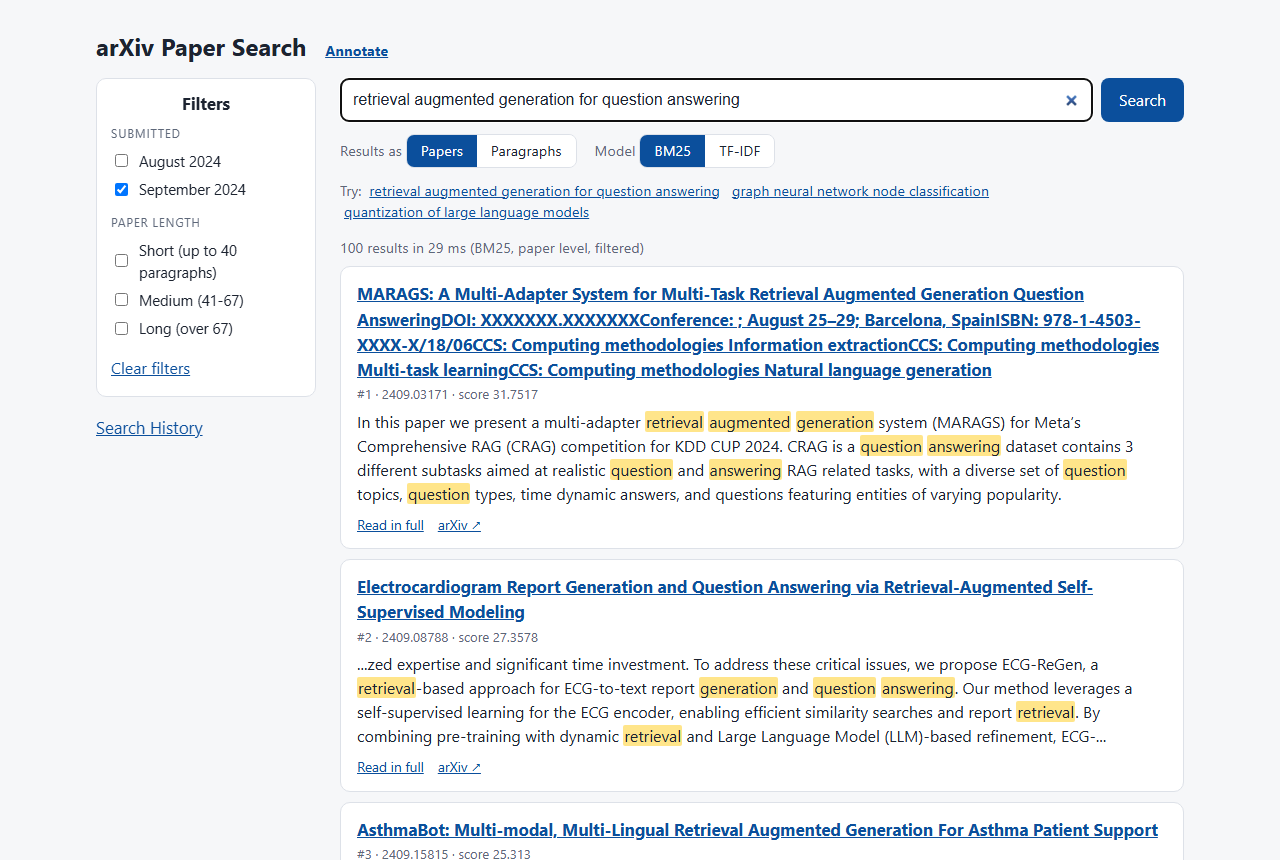
\includegraphics[width=\columnwidth]{interface.png}
\caption{The search interface: filter panel and search-history link (left), query box with model and level toggles (top), and highlighted results. Here the query is restricted to September 2024 papers.}
\label{fig:ui}
\end{figure}

\subsection{Evaluation protocol}
Metrics are computed per query and averaged over the 250 Study queries: nDCG and nDCG@5 with linear gain (ideal ranking from all judged documents); MRR; Precision@5; and Precision@10. MRR and Precision@5 are reported in two variants: lenient (relevance $\ge 1$) and strict (relevance $=2$). We report both variants for Precision@10 as well. Unjudged documents count as non-relevant, and Precision@$k$ always divides by $k$. Because the qrels are sparse, precision has a low ceiling: even a perfect ranking would reach a mean lenient P@5 of only 0.307 for papers and 0.553 for paragraphs. We compare models with a two-sided paired $t$-test and a paired randomization (sign-flip) test with 10{,}000 permutations on per-query differences~\cite{smucker}; $p<0.05$ is marked as significant.

\section{Experimental Results}
% Generated by paper/make_tables.py -- do not edit by hand.
\begin{table*}[t]\caption{Paper-level results on the 250 Study queries (mean over queries; $\ge1$ = Relevant or Partially Relevant counted as relevant, 2 = Relevant only). Best value in bold.}\label{tab:paper-summary}
\small\begin{tabular}{lrrrrrrrr}\toprule
Model & nDCG & nDCG@5 & MRR$_{\ge1}$ & MRR$_{2}$ & P@5$_{\ge1}$ & P@5$_{2}$ & P@10$_{\ge1}$ & P@10$_{2}$ \\\midrule
TF-IDF & 0.3440 & 0.2956 & 0.3081 & 0.2863 & \textbf{0.0912} & 0.0760 & 0.0512 & 0.0428 \\
BM25 & \textbf{0.3596} & \textbf{0.3119} & \textbf{0.3318} & \textbf{0.3096} & 0.0888 & \textbf{0.0776} & 0.0512 & \textbf{0.0432} \\
\bottomrule\end{tabular}\end{table*}

\begin{table*}[t]\caption{Paragraph-level results on the 250 Study queries (mean over queries; $\ge1$ = Relevant or Partially Relevant counted as relevant, 2 = Relevant only). Best value in bold.}\label{tab:paragraph-summary}
\small\begin{tabular}{lrrrrrrrr}\toprule
Model & nDCG & nDCG@5 & MRR$_{\ge1}$ & MRR$_{2}$ & P@5$_{\ge1}$ & P@5$_{2}$ & P@10$_{\ge1}$ & P@10$_{2}$ \\\midrule
TF-IDF & 0.2954 & 0.2156 & 0.2800 & 0.2232 & 0.0928 & 0.0616 & 0.0660 & 0.0396 \\
BM25 & \textbf{0.4148} & \textbf{0.3536} & \textbf{0.4275} & \textbf{0.3557} & \textbf{0.1472} & \textbf{0.0928} & \textbf{0.0888} & \textbf{0.0528} \\
\bottomrule\end{tabular}\end{table*}

\begin{table}[t]\caption{Paired significance tests, BM25 vs.\ TF-IDF on the 250 Study queries (two-sided; $^*$ = $p<0.05$; randomization test with 10{,}000 sign flips). Diff = BM25 $-$ TF-IDF.}\label{tab:sig}
\small\begin{tabular}{llrrr}\toprule Level & Metric & Diff & $p_{t}$ & $p_{rand}$ \\\midrule
paper & nDCG & $+$0.0156 & 0.135 & 0.134 \\
paper & nDCG@5 & $+$0.0163 & 0.212 & 0.212 \\
paper & MRR$_{\ge1}$ & $+$0.0237 & 0.103 & 0.105 \\
paper & MRR$_{2}$ & $+$0.0233 & 0.098 & 0.097 \\
paper & P@5$_{\ge1}$ & $-$0.0024 & 0.565 & 0.707 \\
paper & P@5$_{2}$ & $+$0.0016 & 0.656 & 0.820 \\
paper & P@10$_{\ge1}$ & 0.0000 & 1.000 & 1.000 \\
paper & P@10$_{2}$ & $+$0.0004 & 0.764 & 1.000 \\
\midrule
paragraph & nDCG & $+$0.1194 & $<$0.001$^*$ & $<$0.001$^*$ \\
paragraph & nDCG@5 & $+$0.1380 & $<$0.001$^*$ & $<$0.001$^*$ \\
paragraph & MRR$_{\ge1}$ & $+$0.1475 & $<$0.001$^*$ & $<$0.001$^*$ \\
paragraph & MRR$_{2}$ & $+$0.1326 & $<$0.001$^*$ & $<$0.001$^*$ \\
paragraph & P@5$_{\ge1}$ & $+$0.0544 & $<$0.001$^*$ & $<$0.001$^*$ \\
paragraph & P@5$_{2}$ & $+$0.0312 & $<$0.001$^*$ & $<$0.001$^*$ \\
paragraph & P@10$_{\ge1}$ & $+$0.0228 & $<$0.001$^*$ & $<$0.001$^*$ \\
paragraph & P@10$_{2}$ & $+$0.0132 & $<$0.001$^*$ & $<$0.001$^*$ \\
\bottomrule\end{tabular}\end{table}

\begin{table}[t]\caption{Mean metrics by query difficulty (Study queries; lenient variants; number of queries in parentheses).}\label{tab:difficulty}
\small\begin{tabular}{llrrr}\toprule Level / Model & Difficulty & nDCG@5 & MRR$_{\ge1}$ & P@5$_{\ge1}$ \\\midrule
Paper / TF-IDF & Easy (75) & 0.355 & 0.384 & 0.096 \\
Paper / TF-IDF & Medium (125) & 0.338 & 0.342 & 0.114 \\
Paper / TF-IDF & Hard (50) & 0.099 & 0.109 & 0.028 \\
Paper / BM25 & Easy (75) & 0.383 & 0.410 & 0.101 \\
Paper / BM25 & Medium (125) & 0.365 & 0.382 & 0.109 \\
Paper / BM25 & Hard (50) & 0.073 & 0.090 & 0.020 \\
\midrule
Paragraph / TF-IDF & Easy (75) & 0.382 & 0.468 & 0.149 \\
Paragraph / TF-IDF & Medium (125) & 0.202 & 0.275 & 0.096 \\
Paragraph / TF-IDF & Hard (50) & 0.000 & 0.010 & 0.000 \\
Paragraph / BM25 & Easy (75) & 0.591 & 0.691 & 0.240 \\
Paragraph / BM25 & Medium (125) & 0.352 & 0.438 & 0.149 \\
Paragraph / BM25 & Hard (50) & 0.003 & 0.005 & 0.004 \\
\bottomrule\end{tabular}\end{table}

\begin{table}[t]\caption{Average search time per query (ms) for top-100 retrieval, including query tokenization, excluding index loading, measured in the run that produced the submitted files. Single-threaded Python 3.13 on an Intel Core i7-9750H with 16\,GB RAM.}\label{tab:time}
\small\begin{tabular}{lrrrr}\toprule & \multicolumn{2}{c}{Study} & \multicolumn{2}{c}{Test} \\\cmidrule(lr){2-3}\cmidrule(lr){4-5} Level & TF-IDF & BM25 & TF-IDF & BM25 \\\midrule
Paper & 77.6 & 70.0 & 41.8 & 41.2 \\
Paragraph & 2020.7 & 1682.9 & 2171.7 & 1961.2 \\
\bottomrule\end{tabular}\end{table}


\subsection{Effectiveness}
Tables~\ref{tab:paper-summary} and~\ref{tab:paragraph-summary} give the results at the paper and paragraph level. At the paper level BM25 is slightly ahead on the rank-sensitive metrics (nDCG 0.360 vs.\ 0.344; lenient MRR 0.332 vs.\ 0.308), but the precision metrics are nearly identical and lenient P@5 even favors TF-IDF (0.091 vs.\ 0.089). At the paragraph level BM25 is clearly better on every metric: nDCG rises from 0.295 to 0.415 (+40\%) and lenient MRR from 0.280 to 0.428 (+53\%). The lenient and strict variants agree in direction everywhere except paper-level P@5, where the two models differ on only 24 of the 250 queries. Relative to the precision ceilings above, paragraph BM25 reaches 27\% of the attainable lenient P@5 (0.147 of 0.553), and paper BM25 29\% (0.089 of 0.307).

\subsection{Significance}
Table~\ref{tab:sig} lists the paired tests, and the two tests agree on every comparison. At the paper level no difference is significant; the smallest $p$-value is 0.097 (strict MRR, randomization test), and the two models tie on 143 of 250 queries for nDCG. At the paragraph level all eight differences are significant under both tests with $p<0.001$; BM25 has the higher nDCG on 135 queries, TF-IDF on 26, and 89 are tied. We therefore claim that BM25 outperforms TF-IDF for paragraph retrieval, but not for paper retrieval.

\subsection{Efficiency}
Table~\ref{tab:time} reports the average time to retrieve the top 100 results per query, excluding index loading. Paper retrieval takes 40--80\,ms per query; the Study runs were executed first and most likely include warm-up, which would explain why they are slower than the Test runs. Paragraph retrieval takes 1.7--2.2\,s, because the paragraph index holds 66 times as many documents and the posting lists of common query terms are correspondingly long. BM25 is slightly faster than TF-IDF in every setting. After these runs we replaced the full sort of all scored documents with heap-based top-$k$ selection. On 25 Study queries this produced identical rankings and reduced paragraph search to about 1.1--1.2\,s per query; the submitted files are unchanged.

\section{Result Analysis}
\subsection{By query difficulty}
Table~\ref{tab:difficulty} breaks down the lenient metrics by the Easy/Medium/Hard labels. Performance falls steeply with difficulty. For paragraph BM25, nDCG@5 drops from 0.591 (Easy) to 0.352 (Medium) and 0.003 (Hard); TF-IDF falls from 0.382 to 0.202 and 0.000. BM25's advantage is therefore concentrated on Easy and Medium queries, and on Hard queries both models are essentially at zero. At the paper level the Easy and Medium scores are close (BM25 nDCG@5 0.383 and 0.365), and on Hard queries TF-IDF is slightly ahead (0.099 vs.\ 0.073; 50 queries, not tested for significance).

To explain the drop, we measured \emph{query-term coverage}: the fraction of a query's distinct tokens that appear in its best-covered judged (label 1 or 2) document. At the paragraph level mean coverage is 0.70 for Easy, 0.42 for Medium and 0.16 for Hard queries; at the paper level it is 0.37, 0.28 and 0.16. Hard queries share very few words with their relevant documents, so a purely lexical model has almost nothing to match.

\subsection{Where the models succeed}
Both models place a relevant document at rank 1 for 50 queries at the paper level (20 Easy, 27 Medium, 3 Hard) and 48 at the paragraph level (27 Easy, 21 Medium, none Hard). These queries contain rare, distinctive terms that appear verbatim in the relevant document, so their high IDF dominates the score. Query 2004 asks how axion stars accreting dark matter can be detected via radio astronomy; both models rank first \emph{Radio Lines from accreting Axion Stars}. Query 2005 (charge sequence and flexibility of polyampholytes) retrieves \emph{Structural transitions of a Semi-Flexible Polyampholyte}. At the paragraph level, query 2033 asks how GradTTS generates mel-spectrograms with a score-based decoder, and both models rank first a paragraph beginning ``GradTTS. [41] is a TTS model with a score-based decoder that generates mel-spectrograms''. Across successful queries, the best relevant document covers 0.45 (paper) and 0.63 (paragraph) of the query terms on average, against 0.12 and 0.21 for failed queries.

\subsection{Failure cases}
Neither model retrieves any judged document in its top 100 for 93 queries at the paper level (19 Easy, 37 Medium, 37 Hard) and 69 at the paragraph level (3 Easy, 21 Medium, 45 Hard). We traced the failures to five causes.
\begin{itemize}
\item \textbf{Vocabulary mismatch.} This is the dominant cause, and hard queries are deliberately paraphrased. Query 2011 asks why heart rhythm abnormalities are harder to identify with \emph{wrist-worn optical sensors}; the relevant paper is \emph{Multiclass Arrhythmia Classification using Smartwatch Photoplethysmography Signals}, which shares only \texttt{heart} and \texttt{using} with the query, so BM25 ranks a heart-rate-monitor paper first. Query 2009 describes a \emph{digital helper} and \emph{gaze, body positioning, hand motions}; the relevant paper concerns voice assistants and nonverbal behavior, shares only \texttt{integration}, and loses to a dataset of hand manipulations that matches \texttt{hand} literally. Query 2034 describes a \emph{last-in-first-out data structure} where the relevant paragraph says \emph{stack-based scripting engine}, and query 2012's \emph{rounded spatial limits} means curved mesh edges, so its two relevant papers share no tokens with it at all. Without stemming (\texttt{learning} vs.\ \texttt{learned}) or synonyms, none of these can be bridged.
\item \textbf{Tokenizer losses.} Tokens mixing letters with digits, underscores or accented letters are discarded entirely, so model and benchmark names such as ``3D'', ``L2'' or ``BERT2'' become unsearchable, and ``GPT-4'' is reduced to \texttt{gpt}. LaTeX in queries is tokenized as words: query 2018 (``the map $\iota$ \ldots\ the foliation $\mathcal{F}$'') yields the tokens \texttt{iota}, \texttt{mathcal} and \texttt{f}, and no query token at all occurs in the relevant paper's title and abstract.
\item \textbf{Paper-level representation.} Papers are indexed by title and abstract only. The best relevant paragraph covers far more of an Easy query than the best relevant title and abstract (0.70 vs.\ 0.37 coverage), so paper retrieval misses evidence that lives in the body. Titles and abstracts are also far more uniform in length than paragraphs, which plausibly explains why BM25's length normalization gains little over TF-IDF at the paper level.
\item \textbf{Paragraph granularity and length normalization.} Cosine normalization strongly favors very short paragraphs. TF-IDF's top-10 paragraphs have a median length of 14 tokens, and 60\% have fewer than 20; BM25's have a median of 64 tokens (4\% under 20), and judged relevant paragraphs a median of 78.5 tokens (0.5\% under 20). TF-IDF thus fills its top ranks with headings and fragments that contain a query term but cannot answer the question; BM25's saturating, tunable length normalization avoids this, which is likely the main source of its paragraph-level advantage.
\item \textbf{Partial relevance.} Paragraphs that mention the query topic without answering the question rank highly but earn label 1. Partial labels make up 391 of the 728 paragraph judgments, and strict paragraph MRR is 0.072 lower than lenient MRR for BM25. For queries 2005 and 2016, BM25's rank-1 paragraph is only partially relevant even though the paper-level match is fully relevant.
\end{itemize}

\subsection{Data noise}
The collection was extracted with rule-based cleaning, and we measured the following noise. All counts come from a scan of the 34{,}308 JSON files.
\begin{itemize}
\item \textbf{Malformed records and missing fields.} No file is malformed, and every paper has a title, a non-empty abstract and at least one paragraph. However, 35 abstracts are under 50 characters and hold the wrong text, such as ``Abstract:'' alone or an author list. Titles are noisier: by a pattern count, 4{,}069 titles (11.9\%) have template metadata appended, such as ``Preprint:'' (982), ``Thanks:'' footnotes with author e-mails (942), ``Conference:'' (751), ``DOI:'' (514) or ``CCS:'' (199), and 3{,}544 titles exceed 200 characters. Examples are ``\ldots Question AnsweringDOI: XXXXXXX.XXXXXXXConference: \ldots CCS: Computing methodologies \ldots'' and ``\ldots Semi-Flexible PolyampholytePreprint: APS/123-QED''. Because titles are indexed, this metadata adds spurious terms such as \texttt{conference}, \texttt{computing} and \texttt{methodologies} to the paper-level index.
\item \textbf{Short paragraphs.} No paragraph is empty, but 14{,}975 (0.7\%) are under 50 characters and 617 under 20. Examples are a lone ``$\ast$'' (247 times), the end-of-proof mark ``$\blacksquare$'' (135 times), and headings like ``Step 2: Estimates for the uniform upper bound.'' These are exactly the fragments that cosine-normalized TF-IDF over-ranks.
\item \textbf{LaTeX and math.} About 1.37 million paragraphs (60\%) contain inline LaTeX, such as \verb+$\|r(t)\|_{H^{2}}\leq C_{T}$+, by a regular-expression count that also matches some non-math uses of \$. Display equations were removed entirely, leaving broken sentences such as ``Let and where $\tau=\ldots$. For $j=1,2,\cdots,k$, denote For later''. Command names such as \texttt{mathcal} or \texttt{frac} then enter the index as terms.
\item \textbf{Repeated boilerplate.} 609 distinct paragraphs occur five or more times, totaling 11{,}903 copies. Most are conference checklist answers or disclosure statements, such as ``Guidelines: The answer NA means that the paper does not include experiments.'' (255 times) and ``The authors declare no competing interests.'' (232 times). They carry no topical content but can match generic query words like \texttt{experiments} or \texttt{data}.
\end{itemize}
Curly apostrophes are stored correctly (U+2019), and only 13 paragraphs contain the Unicode replacement character, so encoding errors are rare.

\subsection{Strengths and weaknesses}
Both models are fast at the paper level (under 80\,ms per query), transparent, and need no training data, and their scores can be explained term by term through highlighting in the interface. BM25 is the better default: its length normalization makes it robust to the extreme range of paragraph lengths, giving a significant 40\% nDCG gain over TF-IDF at the paragraph level. The shared weakness is lexical matching. On the 50 Hard Study queries the best relevant document contains on average only 16\% of the query terms, and both models score nDCG@5 of at most 0.099 on them at either level. Paragraph search is also slow for interactive use (1--2\,s per query in pure Python), and the index takes several gigabytes of memory.

\section{Conclusion and Future Work}
We implemented TF-IDF and BM25 from scratch over a shared tokenizer and index, evaluated them on 250 Study queries at paper and paragraph level, and built a search interface and annotation workflow around them. BM25 significantly outperforms TF-IDF for paragraph retrieval, mainly because cosine normalization over-rewards very short paragraphs, while at the paper level the two models are statistically tied; both fail on paraphrased hard queries. Future work includes stemming or lemmatization; a tokenizer that keeps numerals, hyphenated names and accented letters; removing boilerplate, fragments and LaTeX markup before indexing; indexing full paper text or weighted fields for paper retrieval; tuning $k_1$ and $b$ on \texttt{Train.json}; query expansion; and the neural and LLM-based retrieval planned for Phases 2 and 3, which target exactly the vocabulary mismatch that limits these baselines.

\begin{thebibliography}{9}
\bibitem{bm25} Stephen Robertson and Hugo Zaragoza. 2009. The Probabilistic Relevance Framework: BM25 and Beyond. \emph{Foundations and Trends in Information Retrieval} 3, 4 (2009), 333--389.
\bibitem{iir} Christopher D. Manning, Prabhakar Raghavan, and Hinrich Sch\"utze. 2008. \emph{Introduction to Information Retrieval}. Cambridge University Press.
\bibitem{smucker} Mark D. Smucker, James Allan, and Ben Carterette. 2007. A Comparison of Statistical Significance Tests for Information Retrieval Evaluation. In \emph{Proc.\ CIKM}. 623--632.
\bibitem{hearst} Marti A. Hearst. 2009. \emph{Search User Interfaces}. Cambridge University Press.
\end{thebibliography}

\end{document}
